\documentclass{article}
\usepackage{graphicx}
\usepackage{float}
\usepackage{booktabs, 
            makecell, multirow, tabularx}
\usepackage{xcolor}

\title{derivative's}

\begin{document}


\section{Defining average and instantaneous rates of change at a point}
\subsection{Derivative as a concept:}
\noindent
    Derivative is defined as the instantaneous rate of change at a point, 
    or the slope of a tangent line at that point.\\
    which is defined as the \(\lim_{x\to0}\frac{dy}{dx} = f'(x)\).
\subsection{Secant lines and average rate of change:}
    the average rate of change between two points in an interval $[a, b]$ of a curve is defined as the slope of the secant line that connects these points.\newline \newline
    example: \newline \newline

\begin{figure}[ht]
    \centering
    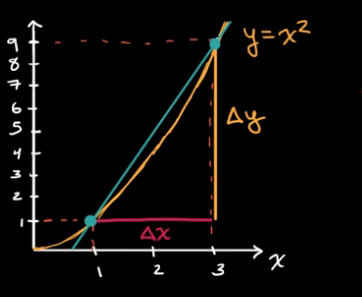
\includegraphics[bb=0 0 360 297, width=0.7\textwidth]{images/secant_line.png}
    \caption{secant line}\label{fig:secant line} 
\end{figure}


\section{Defining the derivative of a function and using derivative notation}
\subsection{Formal definition of the derivative as a limit:}
    h represent some distance more than x. 
    the derivative of a point \(x_0\) formally defined as 
    
   \large \[f'(x_0) = \lim_{h\to0}\hspace{4pt}\frac{f(x_0 + h) - f(x_0)}{h}\]

\subsection{Alternate form of the derivative: }
    the derivative of a point \(x_0\) in alternate form is written as
    
    \large \[f'(x_0) = \lim_{x\to x_0}\hspace{4pt}\frac{f(x) - f(x_0)}{x - x_0}\]
\section{Connecting differentiability and continuity}
\subsection{Differentiability and continuity}
    \begin{itemize}
        \item if f (x) is differentiable at \(x = c\), then f (x) is continuous at \(x = c\)
        \item if f (x) is not continuous at \(x = c\), then f (x) is not differentiable at \(x = c\)
        \item if f (x) is not differentiable at a point, then f (x) may or may not be continuous at that point.
    \end{itemize}
\section{Power rule}
    let the function \large \(f(x) = x ^ n, n\neq 0\), the derivative of \(f(x)\) is given according to the power rule as \large \[f'(x) = nx^{n-1}\]
\section{Derivative rules: constant, sum, difference and constant multiple}
\subsection{Basic rules}
    \begin{itemize}
        \item let A be a constant then \(\frac{d}{dx}[A] = 0\).
        \item let \(f(x)\) be a defined function then: \[\frac{d}{dx}[Af(x)] = A\frac{d}{dx}[f(x)] = Af'(x)\]
        \item let g (x) be a defined function then: \[\frac{d}{dx}[f(x) + g(x)] = \frac{d}{dx}[f(x)] + \frac{d}{dx}[g(x)] = f'(x) + g'(x)\]
    \end{itemize}

\section{Derivatives of \(\cos(x)\), \(\sin(x)\), \(e^x\) and \(\ln (x)\)}
\subsection{Derivatives of \(\sin(x)\) and \(\cos(x)\)}
    \begin{itemize}
        \item \(\frac{d}{dx}[\sin(x)] = \cos(x)\)
        \item \(\frac{d}{dx}[\cos(x)] = -\sin(x)\)
    \end{itemize}
\subsection{Derivative of \(e^x\)}
    \(\frac{d}{dx}[e^x] = e ^ x\)
\subsection{Derivative of \(\ln (x)\)}
    \(\frac{d}{dx}[\ln (x)] =\frac{1}{x}\)
\section{The product rule}
    \[\frac{d}{dx}[f(x)g(x)] = f'(x)g(x) + f(x)g'(x)\]
\section{The Quotient rule}
    \[\frac{d}{dx}\left[\frac{f(x)}{g(x)}\right] = \frac{\frac{d}{dx}[f(x)] \cdot g(x) - f(x) \cdot \frac{d}{dx}[g(x)]}{{g(x)}^2}\]
\section{Derivatives of  \(\tan(x)\) and \(\cot(x)\)}
    tan (x): 
        \[\frac{d}{dx}[\tan(x)] = \frac{d}{dx} \left[ \frac{\sin(x)}{\cos(x)} \right] = \frac{\cos(x) \cdot \cos(x) + \sin(x) \cdot \sin(x) }{\cos{x}^2 } = \frac{1}{\cos{x}^2} = \sec{x}^2 \]
    cot (x): 
        \[\frac{d}{dx}[\cot(x)] = \frac{d}{dx} \left[ \frac{\cos(x)}{\sin(x)} \right] = \frac{-\sin(x) \cdot \sin(x) - \cos(x) \cdot \cos(x) }{\sin{x}^2 } = -\frac{1}{\sin{x}^2} = -\csc{x}^2 \]
\section{Chain rule}
      \[\frac{d}{dx}[f\Bigl(g(x)\Bigr)] = f'\Bigl(g(x)\Bigr) \cdot g'(x)\]
\section{The chain rule: further practice}
    \subsection{Derivative of \(a^x\)(for any positive base a)}
    let \(a = e^{\ln a}\) then: 
    
    \[\frac{d}{dx}[a^x] = \frac{d}{dx}\Bigl[{\Bigl(e^{\ln a} \Bigr)}^{x}\Bigr] = e^{(\ln a)\cdot x} \cdot \ln a = (\ln a) \cdot a^{x}\] 

    \subsection{Derivative of \( \log_a x\) (for any positive base \(a \neq 1\))}
    let \(\frac{d}{dx}[\ln x] = \frac{1}{x}\) and \(\log_a b = \frac{\log_c b}{\log_c a}\) then: 
    \[\frac{d}{dx}[\log_a x] = \frac{d}{dx}\Bigl[\frac{1}{\ln a} \cdot \ln x \Bigr] = \frac{1}{\ln a} \cdot \frac{d}{dx}[\ln x] = \frac{1}{(\ln a)x} \] 
    \subsection{Proving the chain rule}
        \begin{itemize}
            \item \(u(x)\) continuous at \(x = c\) implies that \(\Delta u \to 0\) as \(\Delta x \to 0\)
            \item \(u(x)\) is continuous \(\iff \lim_{x \to c} u(x) = u(c) \equiv \lim_{x \to c}(u(x) - u(c)) = 0\) 
        \end{itemize}
        we have: 
        \begin{itemize}
            \item \(\Delta u = u(x) - u(c)\)
            \item  \(\Delta x = x - c\)
            \item \(\lim_{\Delta x \to 0} \Delta u = 0\)
        \end{itemize}

        \begin{figure}[ht]
            \centering
            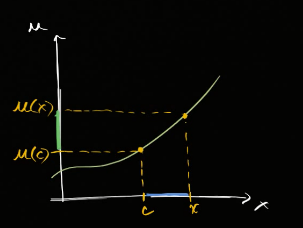
\includegraphics[bb=0 0 303 228, width=0.7\textwidth]{images/change_x_change_u_continuous.png}
            \caption{if function u is continuous at x, then \(\Delta u \to 0\) as \(\Delta x \to 0\)}\label{fig:change_x_change_u_continuous}
        \end{figure}
        chain rule prove: 
        
        assume y, u differentiable at x.
        \[\frac{d}{dx}[y(u(x))] = \frac{dy}{dx} = \frac{dy}{dy} \cdot \frac{dy}{dx}\]
        \[\frac{dx}{dy} = \lim_{\Delta x \to 0} \frac{\Delta y}{ \Delta x} = \lim_{\Delta x \to 0} \frac{\Delta y}{\Delta u} \cdot \frac{\Delta u}{\Delta x} =  \Bigl(\lim_{\Delta x \to 0} \frac{\Delta y}{\Delta u} \Bigr) \cdot \Bigl(\lim_{\Delta x \to 0} \frac{\Delta u}{\Delta x} \Bigr) \]
        \[= \Bigl(\lim_{\Delta u \to 0} \frac{\Delta y}{\Delta u} \Bigr) \cdot \frac{du}{dx} = \frac{dy}{dy} \cdot \frac{du}{dx}\]
        \subsection{Implicit differentiation}
            In implicit differentiation, we differentiate each side of an equation with two variables, by treating one of the variables as function of the other.this calls for using chain rule.

            \noindent example differentiating \(x^2 + y^2 = 1\): 

            \noindent we treat y as an implicit function of x 

            \[x^2 + y^2 = 1\]
            \[\frac{d}{dx}(x^2 + y^2) = \frac{d}{dx}(1)\]
            \[\frac{d}{dx}(x^2) +\frac{d}{dx}(y^2) = 0\]
            \[2x + 2y \cdot \frac{dy}{dx} = 0\]
            \[2y \cdot \frac{dy}{dx} = -2x\]
            \[ \frac{dy}{dx} = -\frac{x}{y}\]
        \subsection{Differentiating inverse functions}
            let f (x) a defined function \noindent
            let g (x) be \(g(x) = f^{-1}(x)\) then \(g(f(x)) = x\) and 
            \[\frac{d}{dx}[g(f(x))] = \frac{d}{dx}[x]\]
            \[g'(f(x)) \cdot f'(x) = 1\]
            \[f'(x) = \frac{1}{g'(f(x))}\]
        \subsection{Differentiating inverse trigonometric functions}
            let \[\sin^2 y + \cos^2 y = 1\]
            Inverse sine:\\
                let \(x = \sin y \)
                \[y = \sin^{-1} x\]
                \[\frac{d}{dx}[\sin y ] = \frac{d}{dx}[x]\]
                \[\cos y \cdot \frac{dy}{dx} = 1 \]
                \[\frac{dy}{dx} = \frac{1}{\cos y}\]
                \[= \frac{1}{\sqrt{1 - {(\sin y)}^2}}\]
                \[\frac{d}{dx}[\sin^{-1}(x)] = \frac{1}{\sqrt{1 - x^2}}\]
            Inverse cosine:\\ 
            let \(x = \cos y\) 
                \[y = \cos^{-1} x\]
                \[1 = (-\sin y)\frac{dy}{dx}\]
                \[\frac{dy}{dx} = - \frac{1}{\sin y} = -\frac{1}{\sqrt{1 - P{(\cos y)}^2}} = - \frac{1}{\sqrt{1 - x^2}}\]
                \[\frac{d}{dx}[\cos^{-1} x] = -\frac{1}{\sqrt{1 - x^2}}\]
            Inverse tangent:\\
            let \(\frac{d}{dx}[\tan x] = \sec^{2} x = \frac{1}{\cos^2 x}\)
                \[y = \tan^{-1} x\]
                \[\frac{d}{dx}[\tan y] = \frac{d}{dx}\]
                \[\frac{1}{\cos^{2} y} \cdot \frac{dy}{dx} = 1\]
                \[\frac{dy}{dx} = \cos^{2} y = \frac{\cos^{2} y}{\cos^{2} y + \sin^{2} y} \cdot \frac{\frac{1}{\cos^{2} y}}{\frac{1}{\cos^{2} y }} = \frac{1}{1 + {\frac{\sin y}{\cos y}}^2} = \frac{1}{1 + {\tan y}^2}\]
                \[ = \frac{1}{ 1 + x^2}\]
                \[\frac{d}{dx}[\tan^{-1} x ] = \frac{1}{ 1 + x^2}\]
        \subsection{Calculating higher-order derivatives}
            the second derivative of a function is the derivative of the function's derivative \\
            let \(f(x) = x^3 + 2x^2\).its first derivative is \(f'(x) = 3x + 4x\), the second derivative of \(f(x)\) would be the differentiation of \(f'(x)\) which is:
            \[f''(x) = 6x + 4\]
            Notation for second derivatives: \\
            leibniz's notation for second derivative is \(\frac{d^2y}{dx^2}\) \\ 
            ex: leibniz notation of \(x^3 + 2x^2\) is \(\frac{d^2}{dx^2}(x^3 + 2x^2)\)
\section{Approximating values of a function using local linearity and linearization}
    \subsection{Local linearity}
        let \(f(x)\)  be a  defined function. \\
        let \((a, b)\) a defined point on the graph of the function \(f(x)\). \\ 
        the approximation of the point \(x_0\).is given as 
            \[f(x_0) = L(x_0) = f(a) + f'(a)(x_0 - a)\]
    \subsection{local linearity and differentiability}
        if \(f(x)\) is differentiable at \(x_0\), then \(f(x)\) is locally linear at that point.
\section{ Using L’Hôpital’s rule for finding limits of indeterminate forms
}
    \subsection{L’Hôpital's rule introduction} 
        \begin{itemize}
            \item case 1: \\ \(\lim_{x \to c} f(x) = 0 \) and \(\lim_{x \to c} g(x) = 0\) and \(\lim_{x \to c}\frac{f'(x)}{g'(x)} = L\) then \(\lim_{x \to c} \frac{f(x)}{g(x)} = L\)

            \item case 2: \\ \(\lim_{x \to c} f(x) = \pm \infty \) and \(\lim_{x \to c} g(x) = \pm \infty\) and \(\lim_{x \to c}\frac{f'(x)}{g'(x)} = L\) then \(\lim_{x \to c} \frac{f(x)}{g(x)} = L\)
                
        \end{itemize}
    \subsection{Proof of special case of l'Hôpital's rule}
        if \(f(a) = 0 \), \(g(a) = 0\) and \(f'(a)\), \(g'(a)\) exist. 
        then \\  \[\lim_{x \to a} \frac{f(x)}{g(x)} = \frac{f'(a)}{g'(a)}\] 
        proof: 
            \[\frac{f'(a)}{g'(a)} = \frac{\lim_{x \to a} \frac{f(x) - f(a)}{x -a}}{\lim_{x \to a} \frac{g(x) - g(a)}{x -a}} = \lim_{x \to a} \frac{f(x) - f(a)}{g(x) - g(a)} = \lim_{x \to a} \frac{f(x)}{g(x)}\]
\section{Using the mean value theorem}
    \subsection{mean value theorem}
        for a function \(f\) that's differentiable over an open interval from \((a,b)\), and continuous over the closed interval \([a,b]\)  that there exists a number \(c\) on that interval such that \(f'(c)\) is equal to the function's average rate of change over the interval 
            \[f'(c) = \frac{f(b) - f(a)}{b - a}\]
        graphically the tangent line at c is parallel to the secant line going through a and b.
\section{Extreme value theorem, global vs local extrema, and critical points}
    \subsection{Extreme value theorem}
        \(f\) is continuous function over \([a,b]\) then \\
        \( \exists \) an absolute maximum and and absolute minimum over that interval.  
        \begin{figure}[ht]  
            \centering
            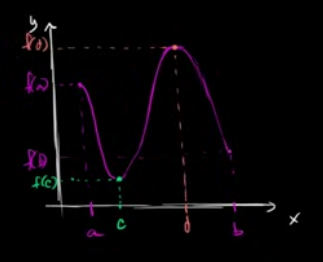
\includegraphics[bb=0 0 323 262, width=0.7\textwidth]{images/minimum_maximum.png}
            \caption{secant line}\label{fig:minimum_maximum}
        \end{figure}
         \[\exists\  c, d \in [a, b] : f(c) \le f(x) \le f(d)\ \forall\ x \in [a,b] \]
     \subsection{Critical points introduction}
        let \(x_0\), \(x_1\), \(x_2\) be non endpoints  maximum or minimum points of \(f(x)\), then the derivative of \(f'(x_0)\), \(f'(x_1)\), \(f'(x_2)\) is either going to be 0 or undefined.\\ 
        A critical point is a point where \(f'\) is equal to 0 or undefined.\\ 
        A critical point is not necessarily an extreme point, the reverse is true.
\section{Determining intervals on which a function is decreasing or increasing}
    \subsection{Increasing and decreasing intervals}
        The intervals where a function \(f(x)\) is increasing (or decreasing) correspond to the intervals where its derivative is positive (or negative) \(f'(x) < 0\) or \(f'(x) > 0\). \\ 
        the derivative of function changes sign at each critical point. 
\section{Using the first derivative test to find  relative (local) extrema}
    \subsection{first derivative test}
        If \(a\) is  min/max value of \(f(x)\) at \(x = a\) then \(a\) is a critical point.\\
        If \(a\) is critical point and in the domain of definition of f.then \(a\) is a maximum point of \(f(x)\), if \(f'(x)\) switches sign from positive to negative as \(f'(x)\) cross \(x = a\).\\  
        If \(a\) is a critical point and in the domain of definition of f.then \(a\) is a minimum point of \(f(x)\), if \(f'(x)\) switches sign from negative to positive as \(f'(x)\) cross \(x = a\). 
        \begin{figure}[ht]
            \centering
            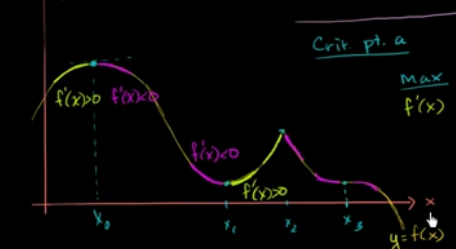
\includegraphics[bb=0 0 456 249, width=0.7\textwidth]{images/first_derivative_test.png}
            \caption{secant line}\label{fig:first derivative test}
        \end{figure}
\section{Using the candidates test to find absolute (global) extrema}
    \subsection{Absolute minima and maxima}
        let \(f(x)\) be defined function over the interval  \(x \in [a, b]\).\\ 
        let \(x_0\), \(x_1\) \(x_2\) be critical points and maximum points of \(f(x)\), where \(f'(x_0) = 0 \ | \ undefined\), \(f'(x_1) = 0 \ | \ undefined\), \(f'(x_2) = 0 \ | \ undefined\).\\
        \(x_1\) is an absolute maximum of \(f(x)\) if and only if \(f(x_1) > f(x_0)\ and \ f(x_1) > f(x_2)\ and \ f(x_1) > f(a)\ and \ f(x_1) > f(b)\).\\
        let \(x_0\), \(x_1\) \(x_2\) be critical points and minimum points of \(f(x)\), where \(f'(x_0) = 0 | undefined\), \(f'(x_1) = 0 | undefined\), \(f'(x_2) = 0  | undefined\).\\
        \(x_1\) is an absolute minimum of \(f(x)\) if and only if \(f(x_1) < f(x_0)\ and \ f(x_1) < f(x_2)\ and \ f(x_1) < f(a)\ and \ f(x_1) < f(b)\).
\section{Determining concavity of intervals and finding points of inflection}
        \subsection{Concavity introduction}
            let \(f(x)\) be  continuous and defined over the interval \([a,b]\).\\ 
            \(f(x)\) is concave downards on a sub interval of \([a,b]\) and has maximum point at \(x_0\) where \(f'(x_0) = 0\) iff: 
            \begin{itemize}
                \item  slope is decreasing: \(f'(x)\) is decreasing
                \item  the second derivative is negative: \(f''(x) < 0 \)
            \end{itemize}
            \(f(x)\) is concave upwards on a sub interval of \([a,b]\) and has minimumpoint at \(x_0\) where \(f'(x_0) = 0\) iff: 
            \begin{itemize}
                \item  slope is increasing: \(f'(x)\) is increasing
                \item  the second derivative is positive: \(f''(x) > 0 \)
            \end{itemize}
            \begin{figure}[ht]
                \centering
                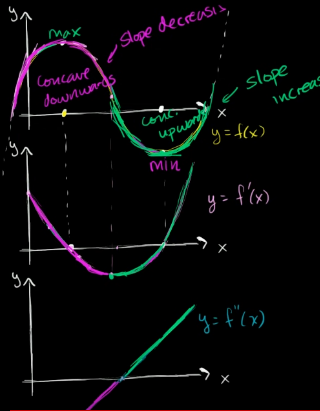
\includegraphics[bb=0 0 320 411, width=0.7\textwidth]{images/concavity.png}
                \caption{secant line}\label{fig:concavity}
            \end{figure}
        \subsection{Inflectoin point introduction}
            Inflection points is a point where the second derivative switches signs \\
            \(x_1\) is an inflection point iff: 
            \begin{itemize}
                \item for \(x < x_1 \): \(f''(x) < 0\) and for \(x > x_1\): \(f''(x) > 0\)
                \item or for \(x < x_1 \): \(f''(x) > 0\) and for \(x > x_1\): \(f''(x) < 0\) 
            \end{itemize}
\section{Second derivative test}
            let \(f'(c) = 0\), \(f'\) exists in neighborhoud around \( x = c\) \\ 
            let \(f''(c)\) exists then \\
            \begin{itemize}
                \item if \(f''(c) < 0\) then \(f\) has  relative maximum at \(x = c\)
                \item if \(f''(c) = 0\) then \(x = c\) is inconclusive 
                \item if \(f''(c) > 0\) then \(f\) has  relative minimum at \(x = c\)
            \end{itemize}
            
\section{Exploring accumulations of change }
        \subsection{Intro to integral calculus}
            let \(f(x)\)  be a  defined function.\\ 
            let \(\delta x_i\) be an infinitesimally small distance of the interval \([a, b]\). \\ 
            the area under the curve of \(f(x)\) between the interval \([a, b]\)
            is represented as: 
                \[\lim_{n \to \infty } \sum_{i=1}^{n} f(x_i) \delta x_i = \int_{a}^{b} f(x)dx\] 
            \(\int_{a}^{b}\) represents the integral of the function \(f(x)\)

            \begin{figure}[ht]
                \centering
                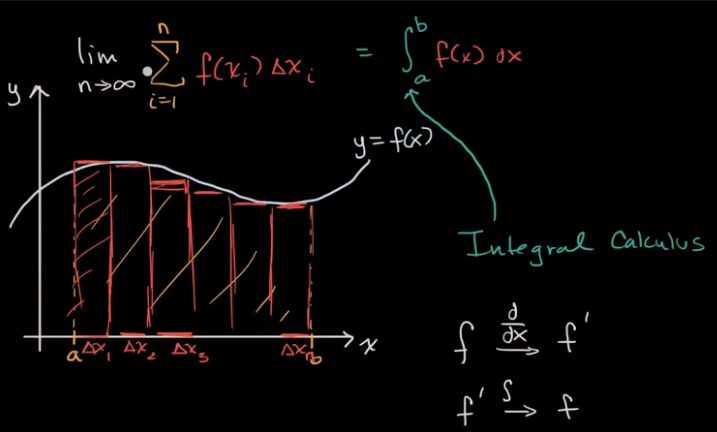
\includegraphics[bb=0 0 717 432, width=0.7\textwidth]{images/intro_integral.png}
                \caption{integrals}\label{fig:integral}
            \end{figure}
        \subsection{Definite integrals intro}
            The area under the curve between the interval \([a,b]\) is denoted as: 
                 \[\int_{a}^{b} f(x)dx\]
            which is the definite integral of \(f(x)\) between two bounds.
        \subsection{Exploring accumulations of change}
            The definite integral can be used to express information about accumulation and net change in applied contexts.
            the definite integral always gives us the net change in a quantity, not the actual value of that quantity\\
            In differential calculus, the derivative \(f'\) of a function \(f\) gives the instantaneous rate of change of \(f\) for a given input.\\
            for any rate function \(f\), its antiderivative \(F\) gives the accumulated value of the quantity whose rate is described by \(f\).\\\\
            \begin{center}
                \begin{tabular}{ c c c } 
                    & Quantity & Rate \\
                    \\
                    \multirow{1}{10em}{Differential calculus } & \(f(x)\) & \(f'(x)\) \\\\ 
                    \multirow{1}{10em}{Integral calculus} & \(F(x) = \int_{a}^{x}f(t)dt\) & \(f(x)\) \\ 
            
                    
                \end{tabular} 
            \end{center}
    \section{Approximating areas with Riemann sums}
        \subsection{RRiemann approximation introduction}
            A Riemann sum is an approximation of the area under a curve by dividing it into multiple simple shapes (like rectangles or trapezoids).\\\\
            In a left Riemann sum, we approximate the area using rectangles (usually of equal width), where the height of each rectange is equal to the value of function at the left endpoint of its base, this type of approximation is considered underestimate.\\
            \begin{figure}[ht]
                \centering
                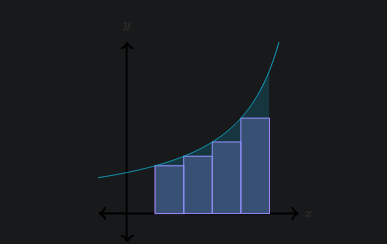
\includegraphics[bb=0 0 387 244, width=0.7\textwidth]{images/left_riem.png}
                \caption{integrals}\label{fig:left Reimann}
            \end{figure} \\ \\
            In a right Riemann sum, the height of each rectangle is equal to the value of the function at the right endpoints of its base.this type of approximation is considered overestimate\\
            \begin{figure}[ht]
                \centering
                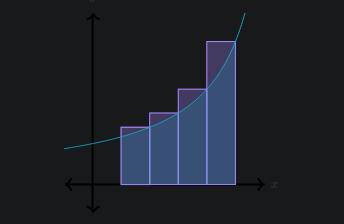
\includegraphics[bb=0 0 355 244, width=0.75\textwidth]{images/right_riem.png}
                \caption{integrals}\label{fig:right Reimann}
            \end{figure} \\
            In a midpoint Riemann sum, the height of each rectangle is equal to the value of the function at the midpoint of its base.\\
            \begin{figure}[ht]
                \centering
                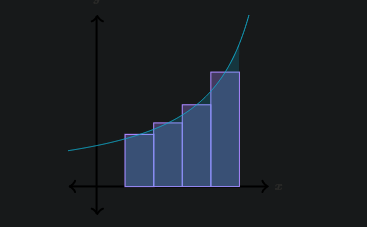
\includegraphics[bb=0 0 355 244, width=0.75\textwidth]{images/mid_riem.png}
                \caption{integrals}\label{fig:midpoint Reimann}
            \end{figure} \\
            We can also use trapezoids to approximate the rea (this is called trapezoidal rule). In this case, each trapezoid touches the curve at both of its top vertices.\\
            \begin{figure}[ht]
                \centering
                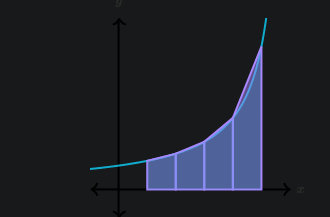
\includegraphics[bb=0 0 355 244, width=0.75\textwidth]{images/trap_rule.png}
                \caption{integrals}\label{fig:trapezoid rule}
            \end{figure} \\
        \section{Riemann sums, summation notation and definite integral notation}
            \subsection{Riemann sums in summation notation}
                Imagine we want to approximate the area under the graph of f over the interval \([a,b]\) with \(n\) equal subdivisions.\\
                Define \(\delta x\): let \(\delta x\) denote the width of each rectangle, then \(\delta x = \frac{b - a}{n}\)\\
                Define \(x_i\): Let \(x_i\) denote the right endpoint of each rectangle, then \(x_i = a + \delta x \cdot i \).\\ 
                Define the area of \(i^{th}\): The height of each rectangle is then \(f(x_i)\), and are of each rectangle is \(\delta x \cdot f(x_i)\).\\
                sum the rectangles: Now we use summation notation to add all the areas. The values we use for i are different for left and right Riemann sums: 
                \begin{itemize}
                    \item When we are writing a right Riemann sum, we will take values of \(i\) from 1 to \(n\)
                    \item However, when we are writing a left Riemann sum, we will take values of \(i\) from 0 to \(n - 1\)(this will give us the value of \(f\) at the left endpoint of each rectangle). 
                \end{itemize}
                \begin{center}
                    \begin{tabular}{ c c  } 
                        Left Riemann sum & Right Riemann sum  \\
                        \\
                        \(\sum_{i=0}^{n-1} \delta x \cdot f(x_i)\) & \(\sum_{i=1}^{n} \delta x \cdot f(x_i)\) \\\\ 
                       
                
                        
                    \end{tabular} 
                \end{center}
            \subsection{Definite integral as the limit of a riemann sum}
                The definite integral of a continuous function \(f\) over the interval \([a,b]\), denoted by \(\int_{a}^{b} f(x)dx\), is the limit of a Riemann sum as the number of subdivisions approches infinity.that is, 
                \[\int_{a}^{b} f(x)dx = \lim_{n \to \infty} \sum_{i = 1}^{n} \delta x \cdot f(x_i)\]

                where  \(\delta x = \frac{b - a}{n}\) and \(x_i = a + \delta x \cdot i\)
        \section{The fundamental theorem of calculus and accumulation functions}
                \subsection{the fundamental theorem of calculus}
                    let \(f\) be continuous function over the interval \([a, b]\).\\ 
                    let \(F(x) = \int_{a}^{x} f(t)dt\), where \(x\) is in \([a,b]\).\\
                    the fundamental theorem of calculus states that: 
                    \[\frac{dF}{dx} = \frac{d}{dx}[\int_{a}^{x} f(t)dt]= f(x)\]
                    \begin{itemize}
                        \item Every continuous function \(f\) has an antiderivative \(F(x)\). 
                        \item the FTOC connects integration and differentiation
                        \item \(F(x)\) is an antiderivative of \(f\).
                    \end{itemize}
        \section{Applying properties of definite integrals}
                \subsection{Negative definite integrals}
                    let \(f\) be continuous defined function.\\ 
                    let \(f([a,b]) < 0\). 
                    then 
                        \[\int_{a}^{b} f(x)dx < 0\]
                \subsection{Definite integrals properties}
                    Sum/Difference: 
                        \[\int_{a}^{b}[f(x) \pm g(x)]dx = \int_{a}^{b} f(x)dx \pm \int_{a}^{b} g(x)dx\]
                    Constant multiple: 
                        \[\int_{a}^{b} k \cdot f(x)dx = k \int_{a}^{b} f(x)dx\]
                    Reverse interval: 
                        \[\int_{a}^{b} f(x)dx = - \int_{b}^{a} f(x)dx\]
                    Zero-length interval: 
                        \[\int_{a}^{a} f(x)dx = 0\]
                    Adding intervals: 
                        \[\int_{a}^{b} f(x)dx + \int_{b}^{c} f(x)dx = \int_{a}^{c} f(x)dx \]
        \section{The fundamental theorem of calculus and definite integrals II}
                \subsection{the fundamental theorem of calculus II}
                    let \(F(x) = \int_{c}^{x} f(t)dt\) and \(F'(x) = f(x)\). 
                    then 
                        \[F(b) - F(a) = \int_{c}^{b} f(t)dt - \int_{c}^{a} f(t)dt = \int_{a}^{b} f(t)dt\]
                    OR 
                        \[\int_{a}^{b} f(t)dt = F(b) - F(a)\]
                \subsection{Antiderivative and indefinite integrals}
                    The antiderivative of \(2x\) is \(\int 2x dx = x^{2} + c\).\\ 
                    ther term \(\int 2x dx \) is called an indefinite integral. 
                \subsection{Proof of the fundamental theorem of calculus}
                    let \(F(x) = \int_{a}^{x} f(t)dt\) where \(a \le x \le b\). 
                        \[F'(x) = \lim_{\delta x \to 0} \frac{F(x + \delta x) - F(x)}{\delta x} = \lim_{\delta x \to 0} \frac{\int_{a}^{x + \delta x} f(t)dt - \int_{a}^{x} f(t)dt }{\delta x} \] 
                        \[= \lim_{\delta x \to 0} \frac{1}{\delta x} \int_{x}^{x + \delta x} f(t) dt\]
                    according to the mean value theorem of definite integral, there exists  a c (where \(x \le c \le x + \delta x\)) such that: \[f(c)\delta x = \int_{x}^{x + \delta x} f(t)dt\]
                    \[f(c) = \frac{1}{\delta x}\int_{x}^{x + \delta x} f(t)dt\]
                    as consequence and according to the squeeze theorem: \\
                        \(c \to x  \) as \(\delta x \to 0\).\\ 
                        \(f(c) \to f(x)\) as  \(\delta x \to 0 \)
                            \[x \le c(\delta x) \le x + \delta x\]
                    \(\lim_{\delta x \to 0 } x = x\), \(\lim_{\delta x \to 0 } c(\delta x) = x\), \(\lim_{\delta x \to 0 } x + \delta x = x\)
\end{document}